\documentclass[leqno,10pt]{article}
\usepackage{algorithm}
\usepackage[noend]{algpseudocode}
\usepackage{hyperref}
\usepackage{float}
\def\Z{\mathbb Z}
\def\Q{\mathbb{Q}}
\def\A{\mathbb{A}}

\makeatletter
\renewcommand{\ALG@name}{Algorytm}
\makeatother

\usepackage{amsmath}
\usepackage{float}
\usepackage{delta}
\usepackage{todonotes}
\usepackage{authblk}

\newcommand{\edge}{\mbox{\rotatebox[origin=c]{90}{\ddagger}}\xspace} 

\def\marg#1{\marginpar{\scriptsize\raggedright#1}}

\begin{document}

\wtyt{Trudność w modelu zawijania białek}


\waut{Marcin Wierzbiński$^{1,2}$, Karolina L. Tkaczuk$^{2}$, Alessandro Crimi$^{2}$}


\marg{[1] Student Wydziału Matematyki, Informatyki i Mechaniki, Uniwersytet Warszawski, [2] Sano Centrum Medycyny Obliczeniowej w Krakowie}

Modelowanie problemów biologicznych za pomocą matematyki czy informatyki to bardzo ciekawy dział. W samym modelowaniu naukowcy jak zwykle chcą pokonać wyzwania, które przed nimi stoją. Jednym z nich jest znalezienie efektywnego algorytmu rozwiązującego tzw. model fałdowania hydrofobowo-polarnego białka. Okazuje się, że ten model ma bardzo wspólnego z informatyką teoretyczną, a sam problem jest trudny do rozwiązania. 

W tym artykule opiszemy bardzo prosty model zawijania białka i jego interpretacje w informatyce teoretycznej. 

\mtyt{Wstęp}
Cząsteczka białka jest tworzona przez ciąg małych cegiełek, znanych jako aminokwasy, które ostatecznie są w stanie zmienić się w natywny kształt białka. Aminokwasy to małe cząsteczki, stanowiące główny budulec białka. Wyróżniamy dwadzieścia aminokwasów, które zwijają się w określoną funkcjonalną strukturę przestrzenną, złożoną z tzw. $\alpha$-heliks, $\beta$-wstążek oraz pętli. Te podstawowe struktury w połączeniu ze sobą tworzą bardziej złożone przestrzennie elementy, jak na przykład $\beta-$kartkę uformowaną z kilku $\beta$-wstążek czy tzw. 'szpilki do włosów' (ang. hairpin loop), która składa się z antyrównoległej struktury $\beta$ podtrzymywanej przez pojedynczy łańcuch polipeptydowy. Omówione konfiguracje przywołują na myśl zbiór koralików, które nawleczone na sznurek łączą się w długi łańcuch. Analogicznie, aminokwasy tworzą długie łańcuchy, które stanowią budulec białek. Interesującą cechą aminokwasów jest, że właśnie one przez sposób, w jaki się ze sobą składają, nadają ostateczny kształt białku, który decyduje o funkcji białka w komórce oraz o tym jak oddziałuje ono z innymi elementami w komórce. 

Istnieje wiele możliwości odtworzenia kształtu białka występującego w naturze. Jako tzw. złoty standard używa się krystalografii, która jest metodą eksperymentalną odtwarzania kształtu przestrzennego białka w danych warunkach. Jest to metoda bardzo czasochłonna i nie zawsze skuteczna, gdy uchwycenie białka bywa niemożliwe, co wynika z faktu, że białko może się okazać bardzo wrażliwe, a w konsekwencji niestabilne w laboratorium. W praktyce oznacza to, że rozpadnie się na kawałki przed odtworzeniem jego kształtu. 
Dlatego zaprzęgnięto metody obliczeniowe do modelowania komputerowego struktur 3D białek. Podstawą takiego modelowania teoretycznego są istniejące już struktury białek (wcześniej eksperymentalnie odtworzone za pomocą krystalografii, zebrane w bazie białek PDB www.rcsb.org). Wraz ze wzrostem możliwości obliczeniowych i coraz szerszym dostępem do nowych metod tworzone są nowe techniki odtwarzania struktur 3D. 
Duże zainteresowanie mediów w ostatnich latach zyskał projekt AlphaFold (\href{https://alphafold.ebi.ac.uk}{alphafold.ebi.ac.uk}), w którym użyta została sztuczna inteligencja (AI) do przewidywania struktur białek.

\mtyt{Model hydrofobowy-polarny(HP)}
Jedną ze znanych uproszczonych metod jest model hydrofobowo-polarny (HP). W tym modelu dwadzieścia aminokwasów jest reprezentowanych jako dwa typy $H$ (aminokwas hydrofobowy) lub $P$ (aminokwas hydrofilowy). Model ten polega na zagięciu danej skończonej sekwencji typów $s \in\{H, P\}^{k}$ o długości $k$ w danej nieskończonej kracie $L=\mathbb{Z}^{3}$ lub $L=\mathbb{Z}^2$ i obliczeniu energii dla tego zagięcia. Każdemu punktowi przypisana jest literka $H$ lub $P$, która jest pobrana z sekwencji $s$.

\marg{Na płaszczyźnie euklidesowej $\mathbb{R}^{3}$ zbiór $\mathbb{Z}^{3} = \{(x, y, z)| \text{ gdzie } x, y, z \in \mathbb{Z}\}$ nazywamy kratą, a jego elementy punktami kratowymi.} 

Zagięciem nazwiemy przekształcenie różnowartościowe $\omega:\{1, \ldots,n\} \rightarrow L$ takie, że sąsiednie liczby odpowiadają sąsiednim punktom z kraty.
\begin{equation}
     1 \leq i<j \leq n: \omega(i) \neq \omega(j)
\end{equation}
Celem rozwiązania problemu składania białek jest znalezienie takiego zagięcia sekwencji aminokwasów w kracie, aby energia całkowita $E_{c}(s , \omega)$ była zminimalizowana. Definicja energii jest zależna od zagięcia sekwencji w kracie i sekwencji typów aminokwasów:
\begin{equation}\label{basic:eng}
    \mathrm{E_{c}}(s, \omega)=\sum_{1 \leq i<j \leq n} E_{(s_{i}, s_{j})} \Delta(\omega(i), \omega(j)),
\end{equation}
stosując wartość równą $-1$ dla sąsiednich wiązań $H \edge H$: 
\begin{equation}
    E_{(s_{i}, s_{j})} = \begin{cases}
        -1 & s_{i}=H \text{ i } s_{j}=H \\ 
        0 & \text{w przeciwnym przypadku}
    \end{cases}   
\end{equation}
i odpowiednią funkcją kodująca liczenie energii dla punktów ze sobą sąsiadujących:
\begin{equation}
    \Delta(\omega(i), \omega(j)) = 
    \begin{cases}
        1 & $\omega(i)$ \text{ i } $\omega(j)$ \text{ są sąsiadami w kracie} \\
        0 &  \text{w przeciwnym przypadku}.
    \end{cases}
\end{equation}
Wzór z $\ref{basic:eng}$ należy tak interpretować, ustaloną sekwencje $s$ zginamy w kracie $L$ przypisując każdemu punktowi literki z $s$. Następnie obliczamy ilość punktów sąsiadujących które mają przypisane dwie literki $H$.
W tradycyjnym modelu pary $H$-ów z sekwencji $s$ nie są liczone jako formujące wiązanie. Dla uproszczenia można dodać pary $H$-ów w liczeniu energii. Uproszczenie w żaden sposób nie wpływa przy ustalonej sekwencji na rozwiązanie. 


\begin{figure}[!htbp]
    \centering
    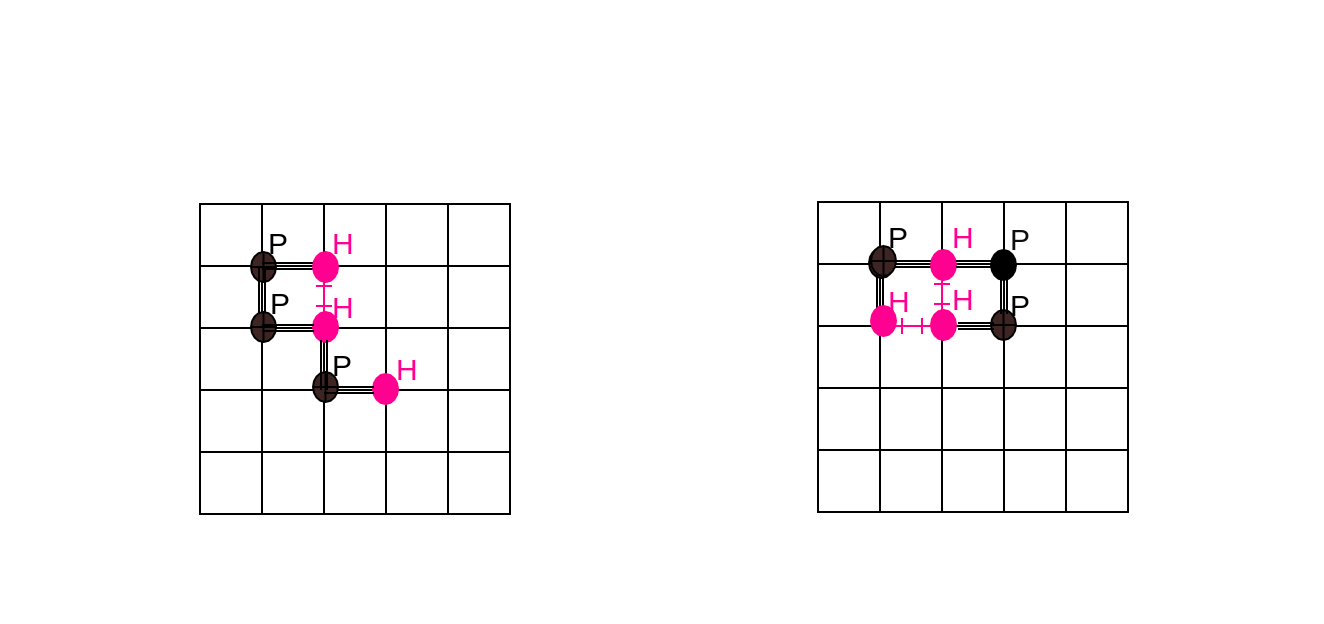
\includegraphics[width=0.9\textwidth]{diagram.png}
    \caption{Przykład zagięcia sekwencji $s={HPPHPH}$ w kracie $L=\mathbb{Z}^{2}$. Po lewej stronie energia całkowita jest równa $-1$, a po prawej stronie $-2$. Co więcej, zagięcie po prawej stronie realizuje globalne minimum energii całkowitej. }
\end{figure}


\textbf{Algorytm losujący}

Jeden z pomysłów, który się nasuwa to myślenie o zagięcie jako o trasie losowego spaceru długości $n$ wzdłuż siatki $L=\mathbb{Z}^{3}$ przy założeniu, że spacer nie przecina swojego dawnego toru, ani nie wraca z punktu wyjściowego. Po angielsku taka droga nazywa się \textit{Self Avoiding Walk}, w skrócie SAW. Losowanie takich spacerów to generowanie zagięcia. W ten sposób można obliczać energię dla zagięcia. Ta metoda  działania nie daje jednak pewności, że algorytm losujący znajdzie globalne minimum energii. Co więcej dla przypadku kraty $\mathbb{Z}^3$ okazuje się, że spacerując w każdym kroku występuje za dużo możliwości wyboru, co sprawia, że trudno zawinąć sekwencje do uzyskania globalnego minimum. 

Samą liczbę zagięć można jedynie oszacować. Podanie dokładnej liczby jest niemożliwe, chyba że dla bardzo małych przypadków $k=\{1,2\}$. Możliwym sposobem oszacowania jest metoda wzrostu zaproponowana przez Ariannę i Marshalla Rosenbluthów. Więcej w artykule opublikowanym w \textit{Delta} $\Delta_{15}^{6}$. Dla małych $n \in \{1,2,3\}$ można policzyć takie zagięcia za pomocą kartki i ołówka. Dla większych wymiarów staje się to niemożliwe. 
\begin{table}[!htbp]
    \centering
    \begin{tabular}{c|c}
      długość sekwencji $k$   &  oszacowanie liczby zagięć \\
       1  & 6 \\
       2  & 30 \\ 
       3  & 150 \\
       4  & 725.4 \\
       5  & 3523.5 \\
       10 & 8863991.25 \\
       15 & 21283727718.75 \\
       20 & 52044761767968.75 \\
    \end{tabular}
    \caption{Oszacowanie liczby zagięć dla kraty $\mathbb{Z}^3$}
\end{table} 
\marg{Więcej jak estymować ilość takich tras jest w artykule opublikowanym w "Delcie" ($\Delta_{15}^{5}$): \href{http://www.deltami.edu.pl/temat/matematyka/zastosowania/2015/04/19/Monte_Carlo_spacery_i_polimery/}{Monte Carlo, Spacery I Polimery prof. Niemiro}}  
Zauważmy, że liczba takich zagięć dla liczby $k>10$ znacząco rośnie. To pokazuje, że problem już dla stosunkowo małych $k$ staje się trudny do rozwiązania. 


\mtyt{Trudność tego modelu}
W informatyce teoretycznej wiele problemów wyraża się jako problemy decyzyjne. Jednak wyżej sformułowany problem jest problemem obliczeniowym - szukamy minimum funkcji energii zadanej tak jak w równaniu \ref{basic:eng}. Warto się zastanowić czy możliwe jest przeformułowanie omawianego problemu w problem decyzyjny, a później w problem obliczeniowy. W tym celu na początku należy ściśle sformułować problem. 


\textbf{Problem zawinięcia sekwencji} 
\newline
Na początku formujemy wejście tak jak w klasycznym algorytmie. 
\newline \textbf{Wejście}: Ustalona sekwencja $s \in \{H,P\}^{k}$, liczbę naturalna $m \in \mathbb{N}$ i kratę $L=\mathbb{Z}^3$. 

Następnie formujemy następujące pytanie  \newline  
\textbf{Pytanie:} Czy istnieje zawinięcie sekwencji $s \in \{H,P\}^{k}$ w kracie $
\mathbb{Z}^3$, gdzie ilość połączeń $H \edge H$ jest przynajmniej $m$? 

Istotne jest tutaj określenie trudności tego pytania, czyli potwierdzenie intuicji, że znalezienie szybkiego deterministycznego rozwiązania nie jest możliwe. Dla zainteresowanego czytelnika techniczne detale można znaleźć w artykule: \textit{'Protein Folding in the Hydrohobic-Hydorplilic HP Model is NP-Complete'} autorstwa Bonniego Bergera i Toma Leightona. 


Warto zauważyć, że algorytm rozwiązujący \textit{problem zawinięcia sekwencji} może zostać wykorzystany w problemie poszukiwania minimalnej energii z równania \ref{basic:eng}. Mając algorytm rozwiązujący problem zwijania się białek, można go uruchomić skończenie wiele razy, zwiększając $m$, by uzyskać informacje o minimalnej energii. W końcu nastąpi moment kiedy odpowiedź będzie przecząca, co wskażę takie $m$, które jest rozwiązaniem problemu obliczeniowego. 

Rozważając problem zawinięcia sekwencji, trudno stwierdzić w jaki sposób dobrać algorytm, aby umiał odpowiedzieć szybko na zadane pytanie. Oczywiście można przetestować bardzo brutalnie wszystkie konfiguracje. Jednak już dla stosunkowo małego rozmiaru sekwencji $k$ problem staje się obliczeniowo niemożliwy do rozwiązania, ponieważ konfiguracje rosną wykładniczo ze względu na $k$, co zostało już przedstawione w tablicy 1. 

Do pokazania trudności stosuje się ciekawy trik, który polega na wprowadzeniu pewnego ogólniejszego problemu decyzyjnego, który się później okaże, jest specjalnym przypadkiem problemu zawinięcia sekwencji. Jeśli ten przypadek okaże się dosyć trudny, to oznacza, że nasz problem także jest trudny. 


\end{document}
